\documentclass[a4paper,11pt,titlepage]{jsarticle}


\usepackage{docmute}
\usepackage{braket}%ブラケット関係のやつ
\usepackage[dvipdfmx]{graphicx}%画像関係のやつ
\usepackage[dvipdfmx]{color}
\usepackage{here}%よくわからん
\usepackage{bm}%ベクトル関係のやつ
\usepackage{amsmath} %数学関係のやつ
\usepackage{listings} %プログラムソースのinclude
\usepackage{color}
% \usepackage{scalefnt}
 
\lstset{ 
  basicstyle={\ttfamily},
  identifierstyle={\small},
  commentstyle={\smallitshape},
  keywordstyle={\small\bfseries},
  ndkeywordstyle={\small},
  stringstyle={\small\ttfamily},
  frame={tb},
  breaklines=true, 
  columns=[l]{fullflexible},
  numbers=left,
  xrightmargin=0zw,
  xleftmargin=3zw,
  numberstyle={\scriptsize},
  stepnumber=1,
  numbersep=1zw,
  lineskip=-0.5ex
} %listingsの設定

\numberwithin{equation}{section} %上手い式の数振り
\setcounter{tocdepth}{3} %subsubsectionまで目次に表示

 
\usepackage{color}

\begin{document}

% input1st
  \section{序論}
  \subsection{高強度レーザー技術の進展}

  1960年代、T.H.Maimanがルビーを用いた固体レーザーの発振に成功した\cite{ft1}ことを皮切りに、レーザー技術は発展し続け、
  1964年にはL.E.Hargroveが開発したモードロックレーザーによってフェムト秒レーザーの発振が達成された\cite{ft2}。
  レーザー発振時の結晶や光学機器の損傷などの問題から、レーザーの高強度化技術は一時停滞していたが、
  1985年に高強度レーザーを得るための極短パルス増幅法である、チャーブパルス増幅法(Chirped Pulse Amplification、CPA)\cite{ft3}
  が開発されたことでレーザーの集光強度(単位:W/cm$^{2}$)は飛躍的に向上し、特に、集光強度が10$^{18}$ W/cm$^{2}$を超えるようになったことで、
  レーザーは電子を光速に近い速度(~0.5 MeV)にまで加速させることが可能となり、電子の相対論領域を扱う新領域の開拓が実現した(図\ref{fig:1}参照)。
  この功績からG.Mourouらは、2018年にノーベル物理学賞を受賞している。

  \begin{figure}[H]
    \begin{center}
      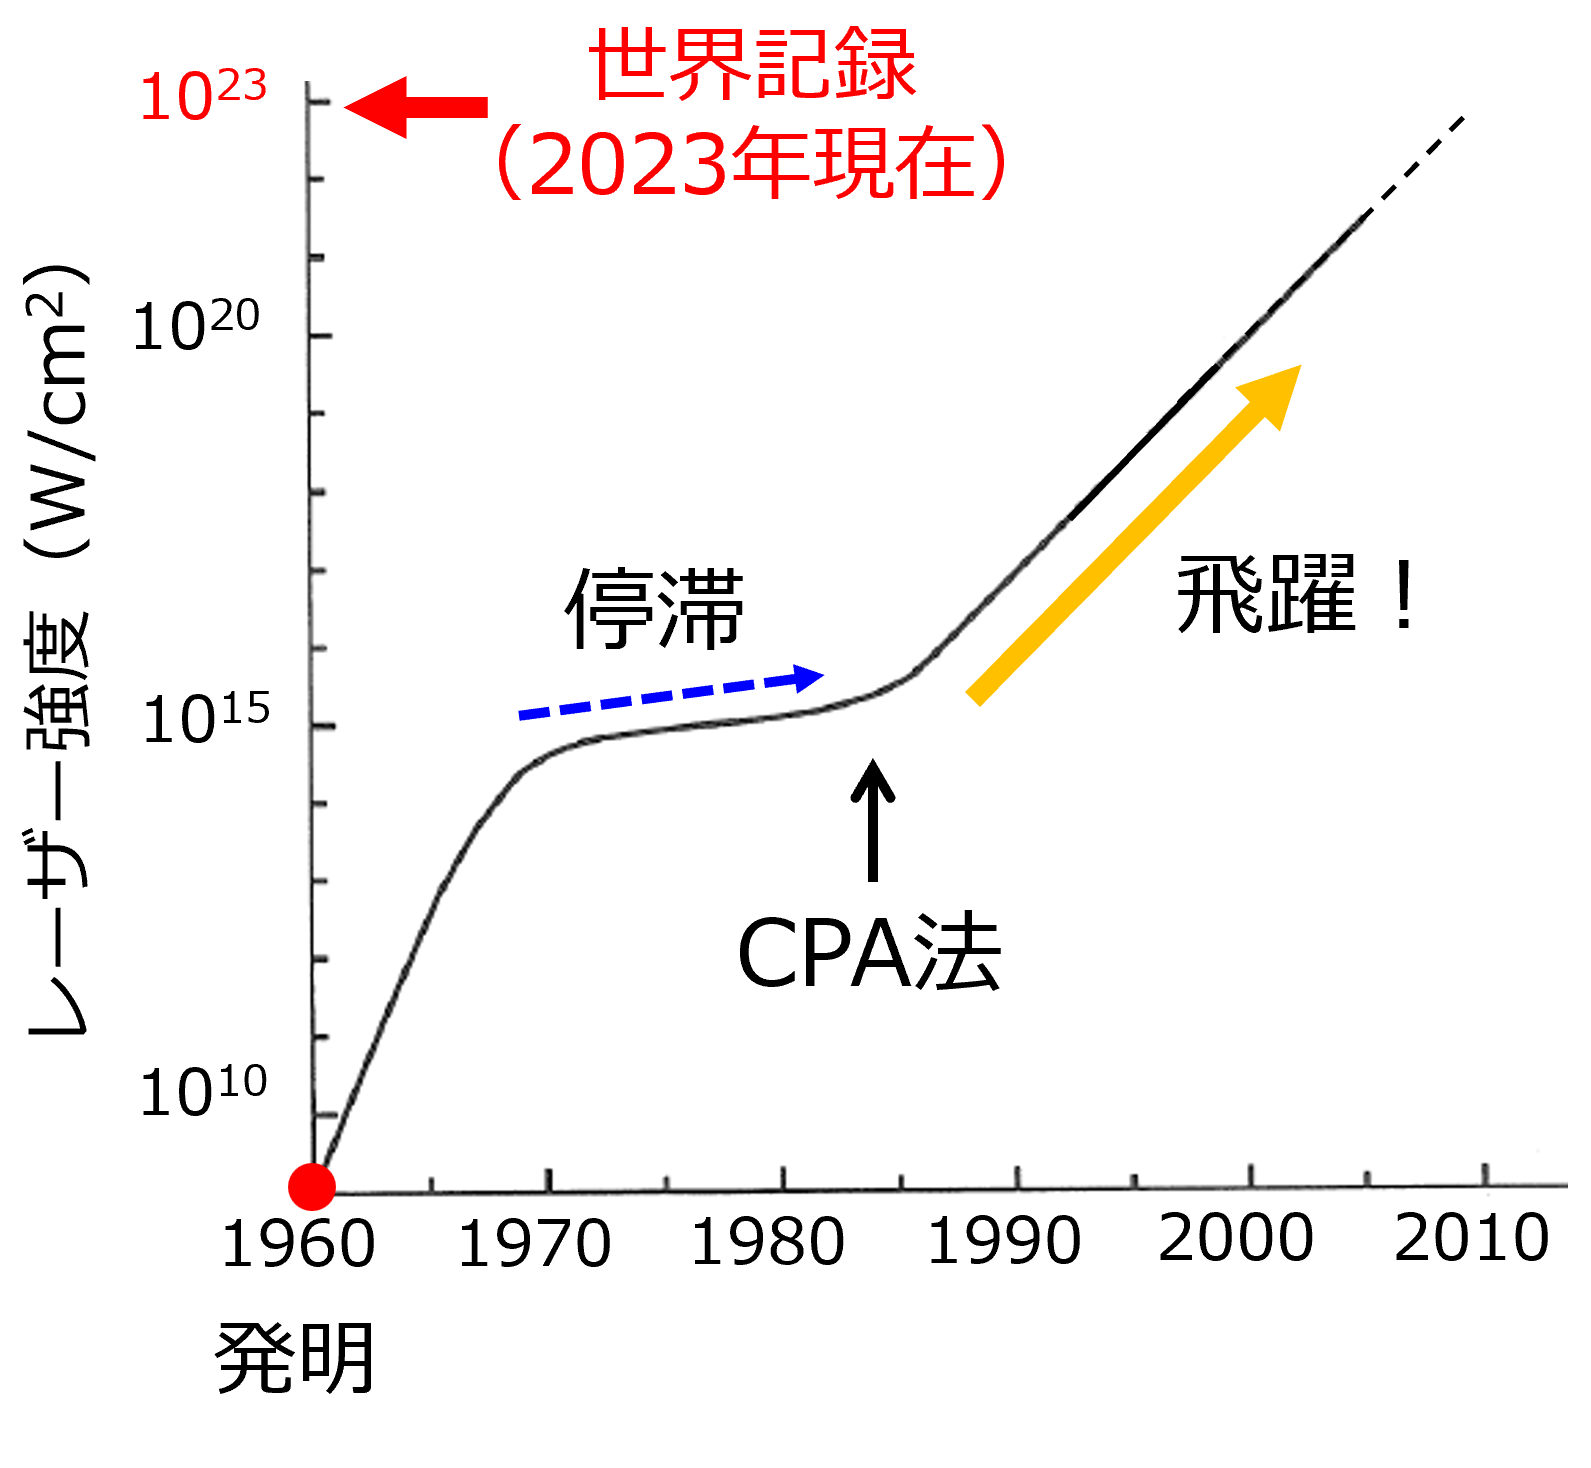
\includegraphics[scale=0.4]{./image/1-laser.png}
      \caption{
        \label{fig:1}
        高強度レーザー技術の発展。横軸は西暦、
        縦軸左は達成されたレーザーの最大集光強度(単位:W/cm$^2$)を示している。
        1985年のチャープパルス増幅法(Chirped Pulse Amplification,CPA法)の開発により、
        レーザー強度は飛躍的に増大している。
        縦軸右はレーザーにより電子が加速された際に得られる電子エネルギー(単位:eV(電子ボルト))を
        表しており、集光強度が10$^{18}$ W/cm$^{2}$で電子は相対論領域(速さ$v$~$c$、$c$:光速)となる。
        P.Gibbon “Short Pulse Laser Interactions with Matter”、Imperial College Press (2005)より引用。
      }
    \end{center}
  \end{figure}

  レーザー強度は、レーザーパルスを出力させる時間(パルス幅)やどれだけの領域に集光させるか(集光径)によって分類可能であり、
  同一のパルスエネルギーに対して、パルス幅が短いほど、また集光径が小さいほどレーザーの集光強度は大きくなる。
  特に物質との相互作用においては、それぞれの領域に応じた相互作用特性を有する。図\ref{fig:pulse}に、
  高強度レーザーにおけるパルス当たりのエネルギー$E$、パルス幅$\tau$、集光強度$I$の関係を示している。
  \begin{figure}[H]
    \begin{center}
      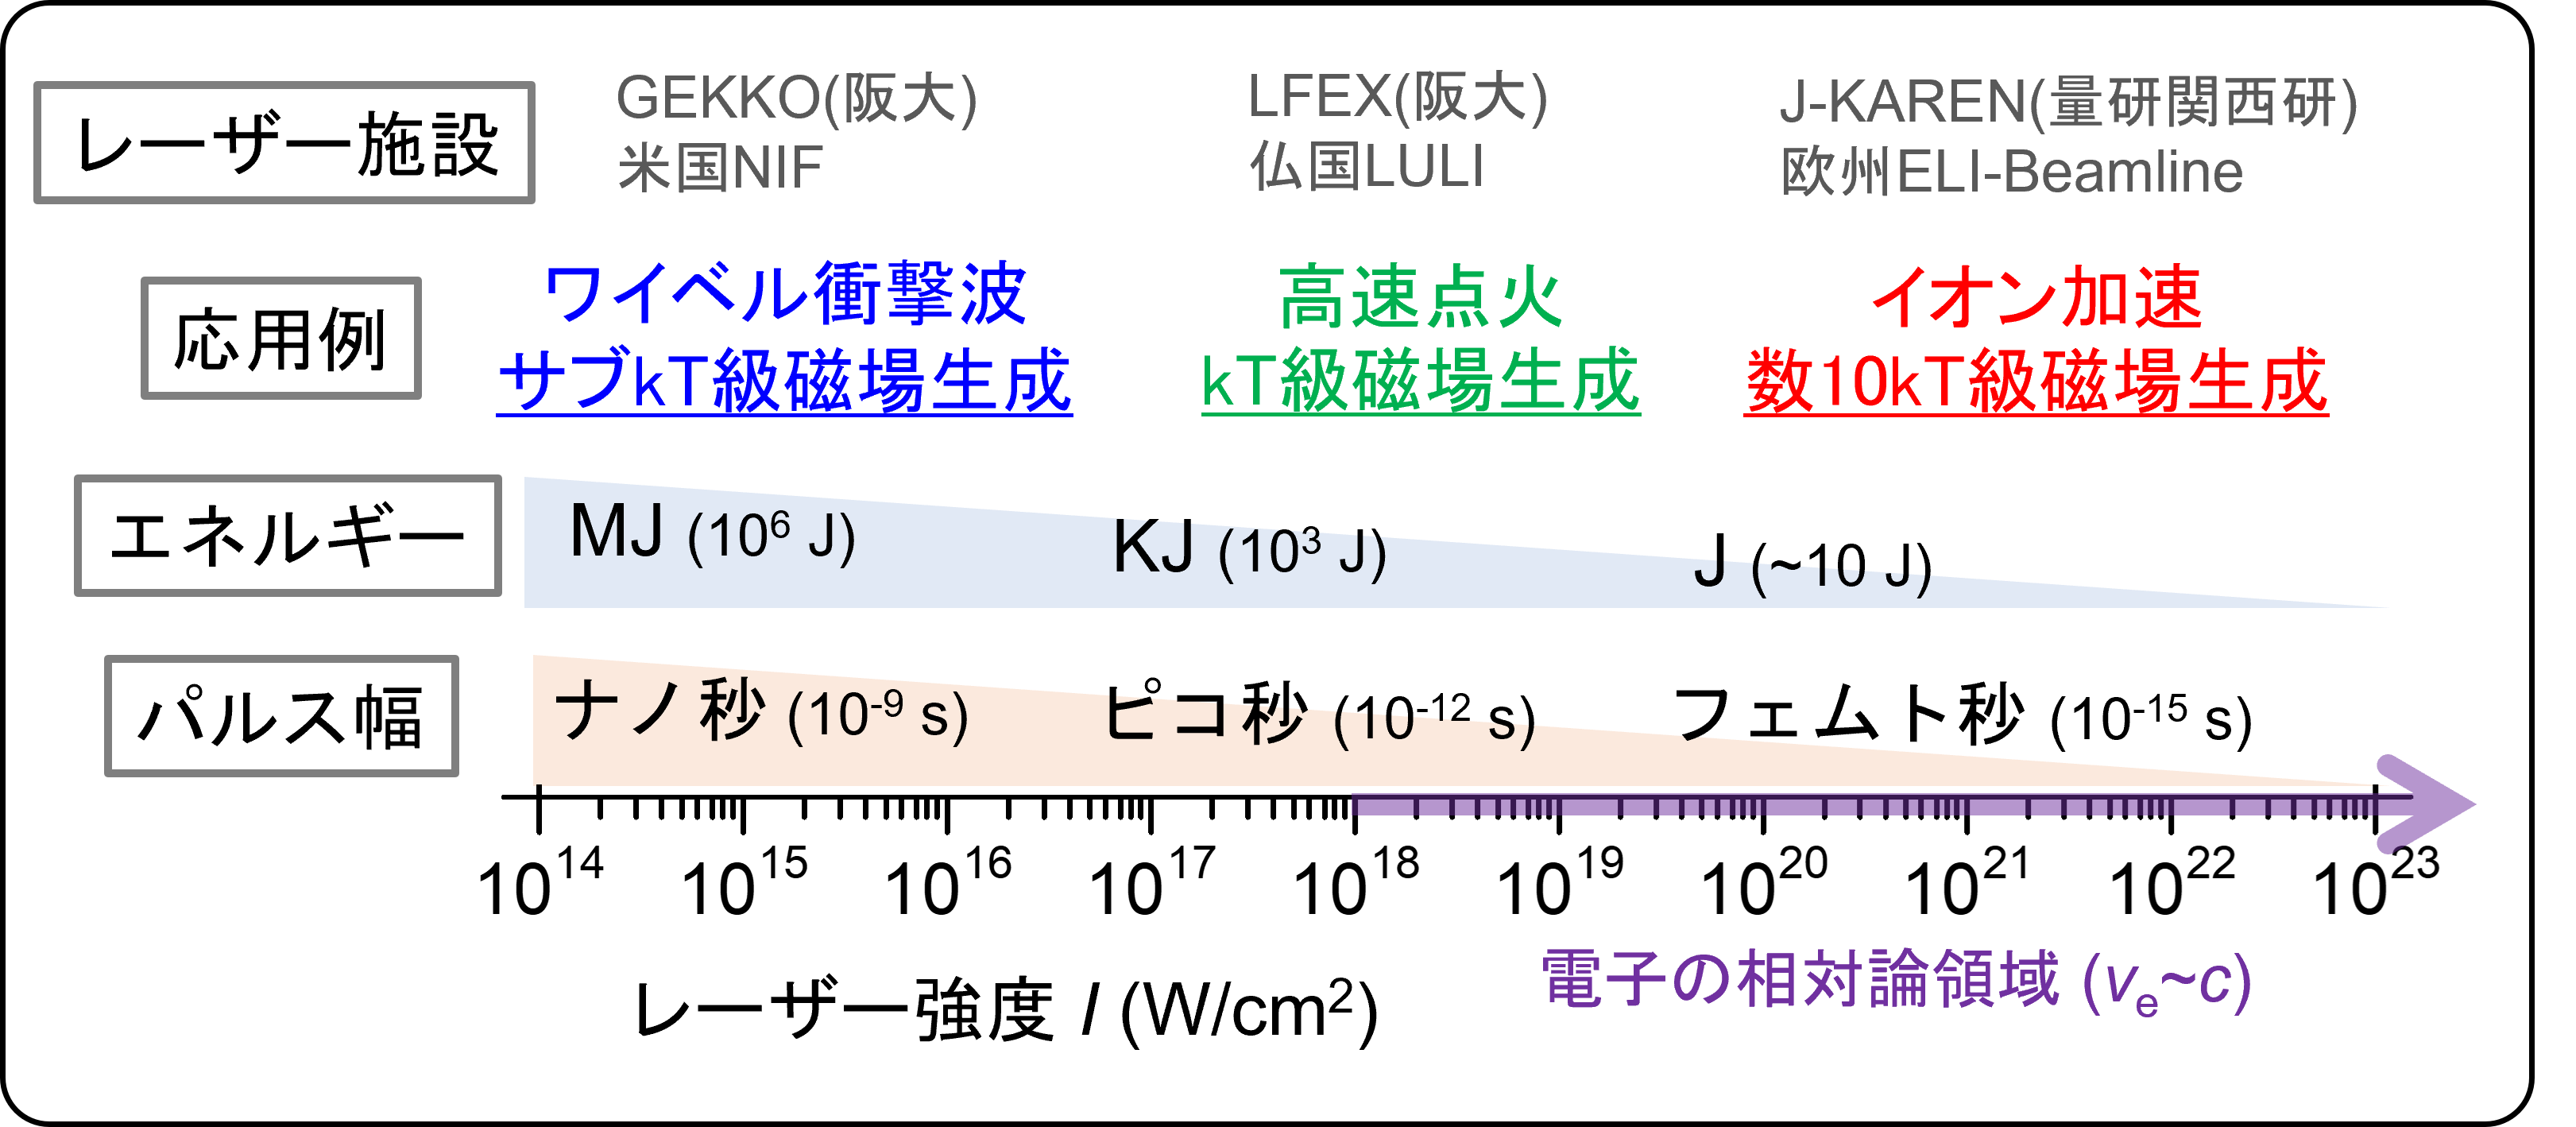
\includegraphics[scale=0.4]{./image/2-pulse.png}
      \caption{
        \label{fig:pulse}
      レーザー強度とエネルギーの関係図。極短パルスのレーザーでは、
      イオン加速、磁場生成などの応用研究の対象が広がる。
      }
    \end{center}
  \end{figure}

  パルス幅がナノ($10^{-9}$)秒領域のレーザー(以下、ナノ秒レーザー)では、MJ(メガジュール)レベルのエネルギーをナノ秒で出力させることで、
  集光強度$I \sim 10^{14-16}$ W/cm$^{2}$が得られる。この領域では、ナノ秒にわたりMJという莫大なエネルギーを照射することが可能であり、
  慣性核融合に向けた実験研究や、高エネルギー宇宙線の生成起源とされるワイベル衝撃波生成を実験室で模擬することを目指した研究(実験室宇宙物理)などに利用されている。
  パルス幅がピコ($10^{-12}$)秒領域のレーザー(以下、ピコ秒レーザー)では、kJ(キロジュール)のエネルギーをピコ秒で出力させることで、
  集光強度$I\sim 10^{18-20}$ W/cm$^2$が得られる。この領域のレーザーは、電子を光速に近い速度にまで加速させることが可能であり、
  物質との相互作用においては電子の相対論領域を扱うこととなる。したがって、相対論的速度での電子運動によりMA(メガアンペア)レベルの電流が駆動され、
  kT(キロテスラ)級の強磁場の生成が可能となる。kTオーダの磁場は、レーザーを用いる手法以外では、100 kgレベルのTNT爆薬の爆発を利用した瞬間的な発生装置等に留まり、
  強磁場を利用した応用研究の枠組みでは、ピコ秒レーザーを用いる方法が有用であることが分かる。
  パルス幅がピコ($10^{-15}$)秒領域のレーザー(以下、フェムト秒レーザー)では、チタン・サファイア結晶を用いた発振が代表的であり、
  数Jのエネルギーをフェムト秒オーダ、かつ光(波長$\lambda \sim 1 \mu$ m)の回折限界に近い数$\mu$m(マイクロメートル)まで集光させることで、
  得られる集光強度は$I \sim 10^{21-22} $W/cm$^{2}$領域に達する。この強度領域のフェムト秒レーザーを物質に照射することで、
  フェムト秒の時間スケールで消失するものの、数$\mu$m$\sim$数10$\mu$mの空間領域に、数10 TV(テラボルト)/mの超強電場、および、中性子パルサーに匹敵する数10kTに達する超強磁場が生成する。
  このような超強電磁場を利用することで、イオンを核子当たり数10$\sim$ MeV領域にまで加速させることで、粒子線がん治療装置の開発に向けた基礎研究や、
  衝撃波加速をはじめとする宇宙での極限現象の解明に向けた研究などが進展している。
  表1に、国内外の主要なレーザー施設、および、主なパラメータを示している。

  
  \begin{table}[H]
    \caption{レーザーの一覧}
    \centering
    \scalebox{0.85}{
      \begin{tabular}{lccccc} \hline \hline
        \multicolumn{5}{c}{レーザーの一覧} \\ \hline
        レーザー & 集光強度 & パルス幅 & 最大エネルギー & 波長 & 出力 \\ \hline 
        激光 XII(日) & $\sim 1\times 10^{19}\ \mathrm{W/cm^{2}}$ 
        & 0.1 $\sim$ 0.4 ns & 250 $\sim$ 1000 J & 527 or 1053 nm & 1 PW \\
        NIF(米) & $\sim 1\times 10^{16}\ \mathrm{W/cm^{2}}$  & 20 ns & 1.8J & 1053 nm & 500 TW \\ \hline
        LFEX(日)  & $ \sim 1\times 10^{19}\ \mathrm{W/cm^{2}}$ 
        & $0.5 \sim 20$ ps 
        & 2.5 kJ & 1053 nm & 2 PW \\ 
        OMEGA EP(米) & $ \sim 6 \times 10^{19}\ \mathrm{W/cm^{2}}$ 
        & $0.7 \sim 100$ ps 
        & 0.5 $\sim$ 2.3 kJ & 1053 nm & 不明 \\ \hline
        J-KAREN(日) & $ \sim 1\times 10^{22}\ \mathrm{W/cm^{2}}$ & 40 fs 
        & 30 J & 810 nm & 1 PW \\ %\hline \hline
        ELI(羅) & $\sim 1\times 10^{23}\ \mathrm{W/cm^{2}}$  & $\sim 17$ fs
        & $\sim$ 34 J & 800 $\sim$ 1030 nm & $\sim$ PW \\ \hline \hline
    \end{tabular}
    }
  \end{table}

  最近では、量子科学技術研究開発機構・関西光科学研究所のJ-KAREN-Pレーザー
  \cite{19,20}などが
  レーザーの最大集光強度$10^{22}\ \mathrm{W/cm^{2}}$の
  フェムト秒極短パルス高強度レーザーを実現している。このようなフェムト秒高強度レーザーを物質に照射することで、
  物質はレーザーのパルス時間スケール(フェムト秒オーダ)で瞬時に電離してプラズマ化するとともに、発生した多数の電子がレーザー光の光圧によりレーザー伝播方向に光速に近い速度にまで加速される。
  これにより、圧力が太陽の中心部の圧力(2000億気圧)の1/10に迫る、100億気圧オーダの高エネルギー密度プラズマが実験室レベルで生成可能である。
 

  \subsection{医療・産業・学術への応用}
  \bf{イオン加速}\\
  \rm
  集光強度が10$^{18}$ W/cm$^{2}$を上回る高強度レーザーを、
  厚さが数10 nmから数$\mu$mのプラスチックや金属等の固体薄膜や、
  大気圧~大気圧の数倍に達する高密度ガスに照射することで、
  これらはフェムト秒のオーダで電離してプラズマ化する。
  このとき、電子はレーザー電場により電場方向に振動しながら、
  ローレンツ力の磁場成分($\bm{v} \times \bm{B}$)を受けてレーザー伝播方向(前方)に運動する。
  一方で、イオンは質量が大きいためレーザー場による運動は無視でき、その場に留まる。
  これにより、前方に運動した電子と残されたイオンとの間にはTV/mに達する超強電場が生成する。
  この電場により、イオンは電子に追随する形で前方に加速される。
  これらの現象は、物質表面のレーザー光照射領域(直径数$\mu$m~数10$\mu$m程度のレーザー集光径の領域)で起こり、
  電場が存在する領域も$\mu$mオーダの非常に局所的であるが、TV/mの電場で$\mu$mのスケールで加速されたイオンは、
  典型的には核子当たり数MeVのエネルギーを得ることになる。
  これは、既存の大型加速器でイオンを加速した場合と比較して10$^{3}$-10$^{4}$倍の加速効率に相当する。
  すなわち、高強度レーザーを用いることで、イオン加速器の小型化が期待できる。\cite{ft6}
  このようなイオン加速手法は、レーザー駆動型のイオン加速手法と呼ばれており、
  レーザー集光強度の増大とともにプラズマ中で生成する電場強度も大きくなり、
  近年達成されつつある集光強度10$^{21-22}$ W/cm$^{2}$の領域では、
  100 TV/mの超強電場の生成が理論的に予測されており、
  これにより100 MeV/uのイオン生成も視野に入っている。\cite{100Mev1,100Mev2,100Mev3}
  したがって、この手法により、医療応用可能とされている200 MeV/uを上回るエネルギーまで短距離で加速できれば、
  これまで少数の大型施設でしか提供できなかった粒子線癌治療などの高度医療に新たな展開をもたらすことができるため、
  TNSA(Target Normal Sheath Acceleration)、\cite{ClarkPRL2000,SnavelyPRL2000,WilksPoP2001,FushsNP2006,HegelichN2006,SchwoererN2006}
  RPA(Radiation Pressure Acceleration, 輻射圧加速)\cite{ft7,ft8,ft9}、
  CSA(Collisionless Shock Acceleration)といった代表的な加速機構\cite{SilvaPRL2004,HaberbergerNP2012,FiuzaPRL2012,FiuzaPoP2013,ZhangPoP2015,WangPoP2016,ChenSR2017,ZhangPRL2017}を中心に、
  世界的に研究が進められている。一方で、これまで実験により得られているイオンの最大エネルギーは
  100 MeV/u に留まるとともに、イオンのエネルギーと実用化に向けたイオンビームの品質(高単色性・高指向性・高フラックス)は
  相反関係を示し、未だ同時達成された例はない。 
  \bf{慣性核融合}\\
  \rm
  レーザーのパルス長がナノ秒領域となると、レーザーの集光強度領域は1015-16 W/cm2となる。
  20Tの種磁場を円筒状チタン内部に(円筒の軸方向に)通した上で、円筒の側面から集光強度1015 W/cm2、
  パルス幅0.5 nsのレーザーを照射することで、円筒をプラズマ化し半径方向に圧縮する。
  このとき、円筒内の空洞が圧縮されることで、ファラデー回転を用いた測定によると、
  種磁場が増強されることで0.8 kTの強磁場が生成され、2 nsにわたり準定常に存在することが実験により報告されている。\cite{kansei}\\
  \bf{実験室宇宙物理}\\
  \rm
  高速プラズマ流による強磁場の生成、およびそれによる(電磁的)無衝突衝撃波は、
  宇宙において普遍的にみられる現象である。ここで、対向する高速プラズマ流がぶつかることで生じるワイベル不安定性(Weibel instability)が、
  衝突面近傍で強い磁場を生成し、この磁場により上述の無衝突衝撃波が形成されると考えられている。
  一方で、高強度レーザーを物質に照射することで生成する宇宙レベルの極限プラズマを実験室で再現する試み(実験室宇宙物理)において、
  ワイベル不安定性の証拠となる「強磁場」の観測は困難な課題となっている。
  C. M. Huntingtonらは、プロトン・ラジオグラフィー法を用いて、レーザー生成対向高速プラズマ流により、ワイベル不安定性に由来する強磁場が生成した証拠を観測することに成功している。\cite{zikken}
 
  \subsection{構造性媒質}
  このように、集光強度が10$^{19-21}$ W/cm$^{2}$領域の高強度レーザーを様々な物質に照射することで生成する数億気圧(Gbar)に達する高エネルギー密度プラズマは、
  同時にプラズマ中に駆動される超強電磁場や大電流とともに、これを利用した高エネルギー粒子加速やレーザー核融合、宇宙レベルの現象など、
  様々な応用研究が期待される。一方、このような過程は、圧力の不均衡に起因した非定常性の強い過渡現象であり、
  それらはレーザーのパルス幅(~慣性時間)程度で散逸することから、応用研究もその時間内に成立するものに限られる。(図\ref{fig:1-3_1}参照)
  \begin{figure}[H]
    \begin{center}
      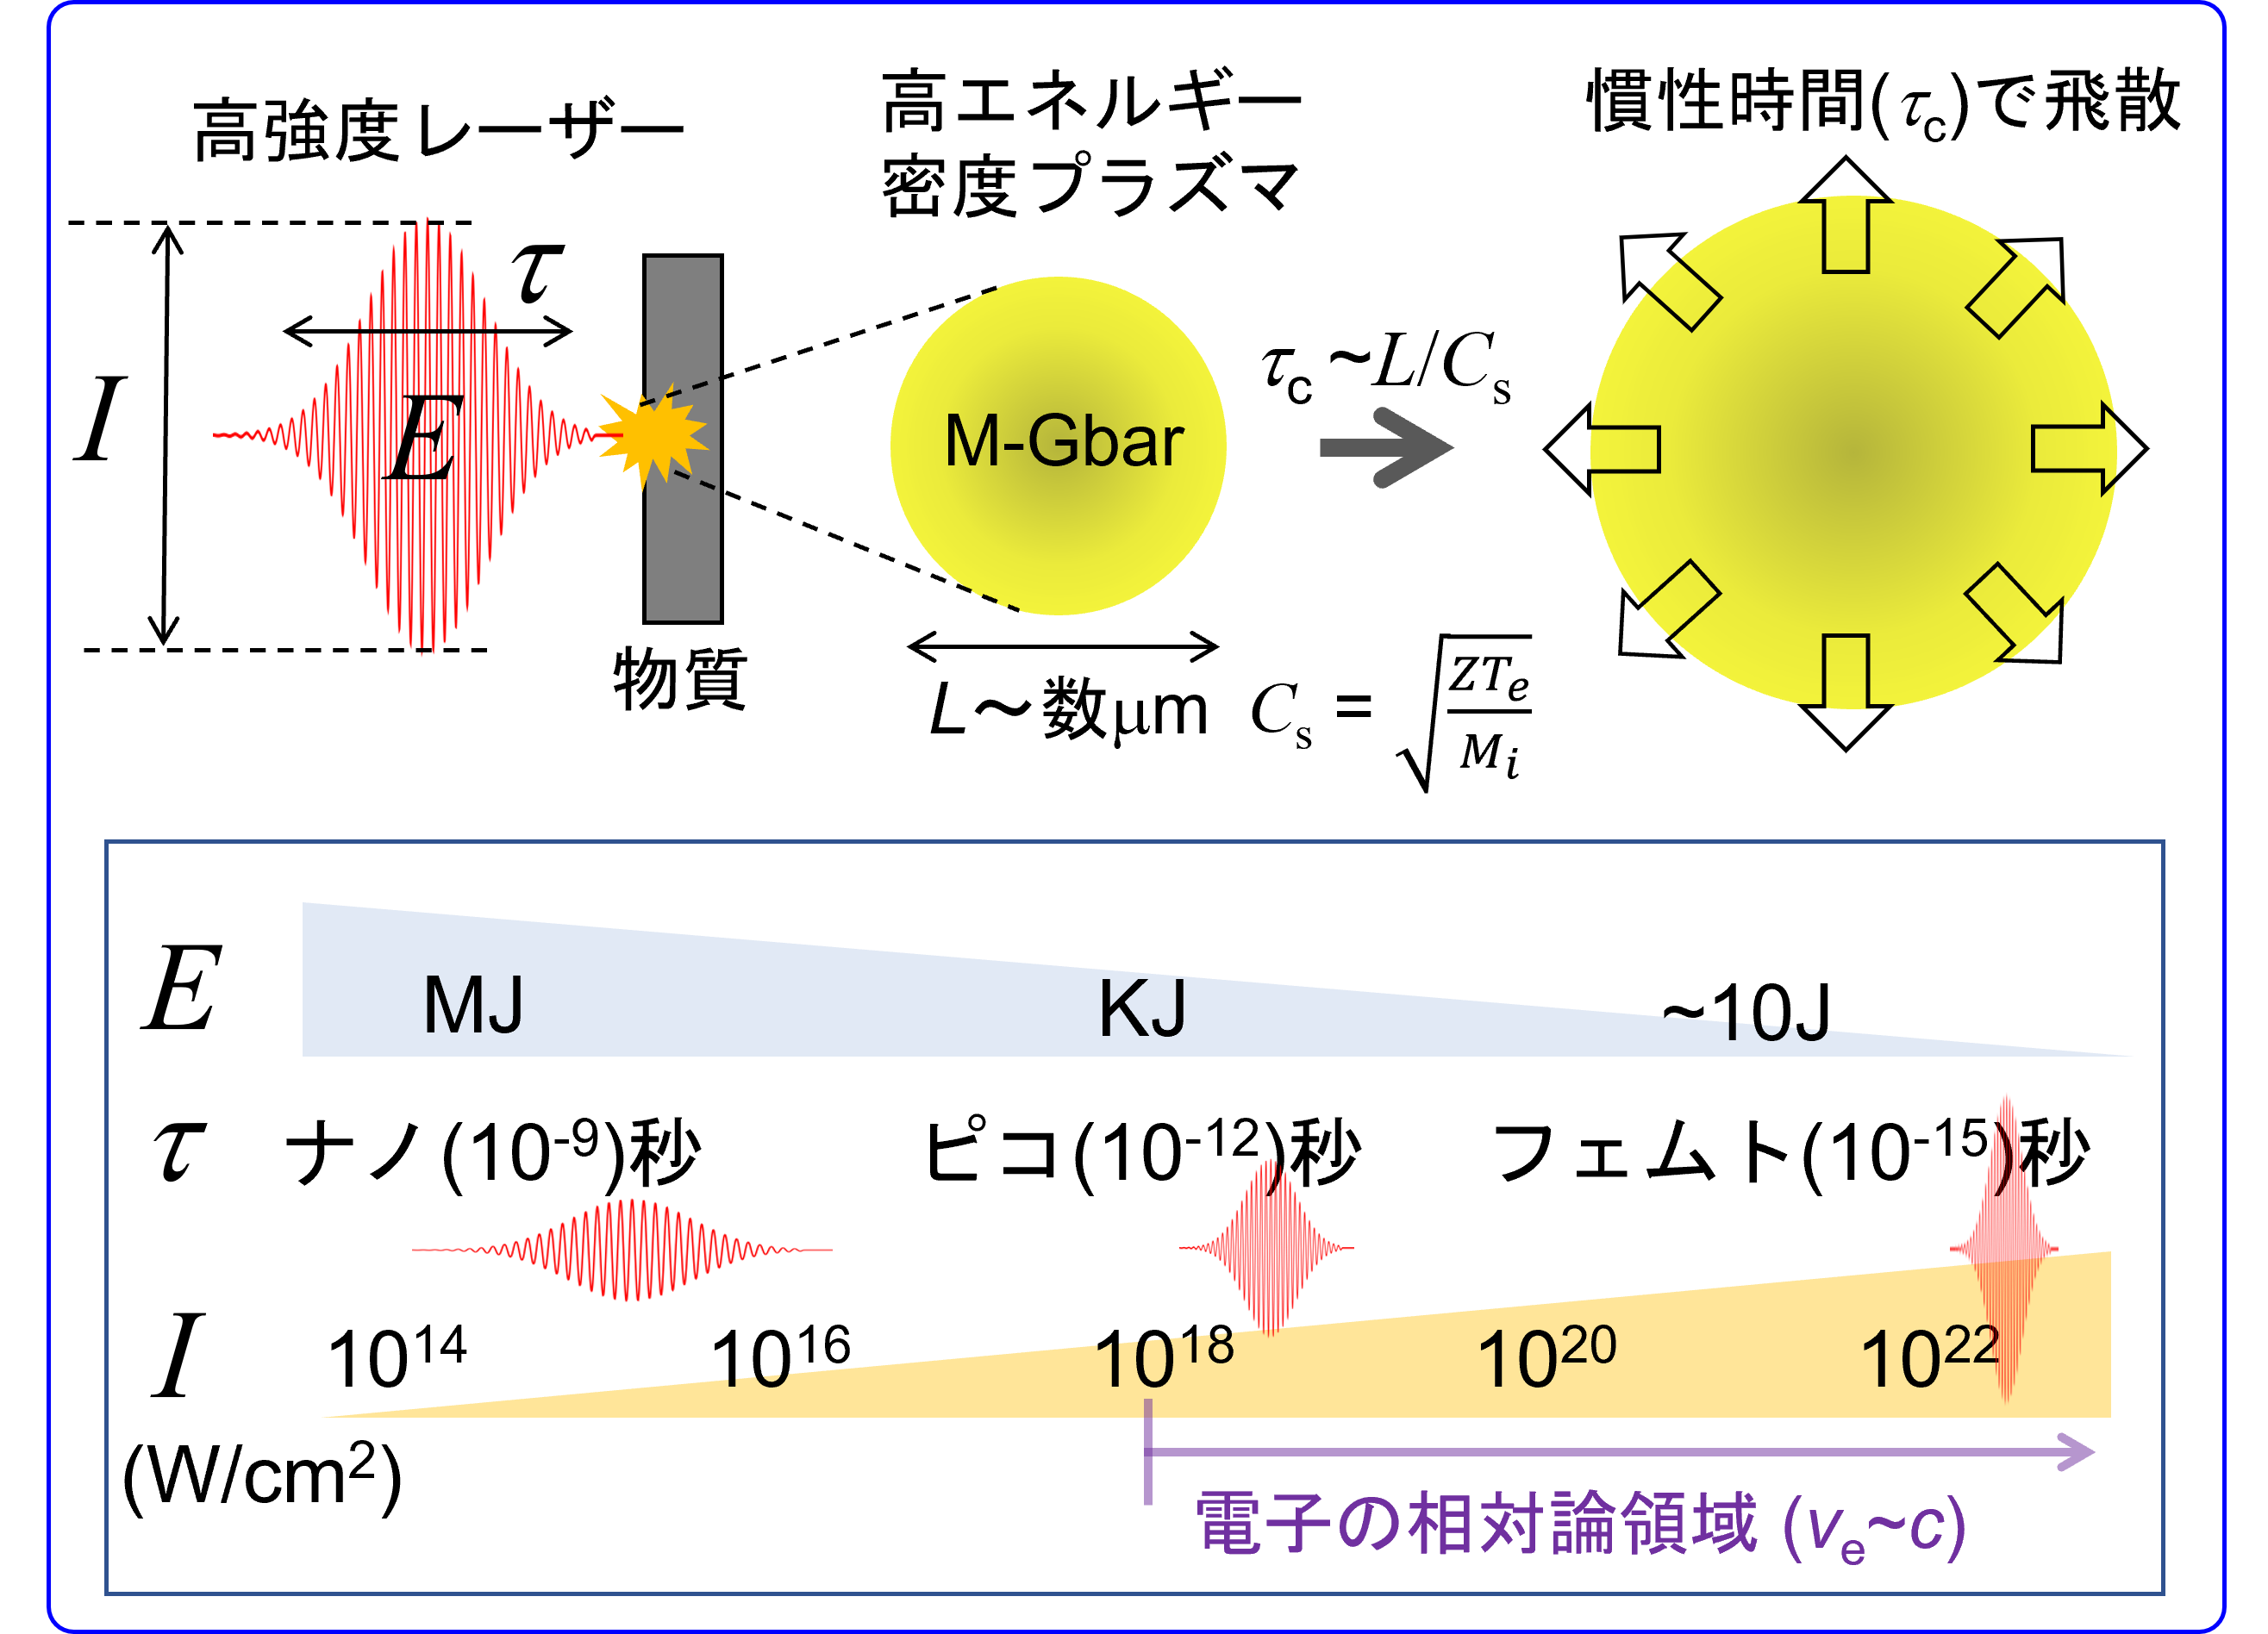
\includegraphics[keepaspectratio,width=\linewidth]{./image/1-3/1-3_1.png}
      \caption{
        \label{fig:1-3_1}
          高強度レーザーを照射されたターゲット。通常、このような過程で生成する高エネルギー密度プラズマは
          慣性時間$\tau_c$程度の時間スケールで飛散し、応用研究の対象はその範囲内で起こりうる現象に限られる。
      }
    \end{center}
  \end{figure}
  これは、逆に、これまで慣性時間程度で飛散していた高エネルギー密度プラズマをこれを超えて長時間“閉じ込める”ことができれば、
  上述の課題を克服して学術・応用研究の枠組みを広げることができる。この着想のもと、当研究室では、高強度レーザーを照射する物質として、
  一般に広く用いられている固体薄膜(厚さ数10$\sim$数100 nmに加工されたプラスチックや金属平板)に対して、物質の形状を球や円柱とすることで、
  比表面積(質量に対する表面積の割合)が増大し、物質表面とレーザーとの相互作用過程を通じて多彩な非線形現象を創出し得ると着想し、
  直径数100 nm$\sim$$\mu$mの粒状固体物質(クラスター)や、直径がサブ$\mu$mで高さが数10$\mu$mオーダの円柱状ケイ素(ロッド)が$\mu$m間隔で複数配列した媒質(ロッド集合体)を
  ターゲットとして選択し、これらに集光強度領域が10$^{19-22}$ W/cm$^{2}$の高強度レーザーを照射する粒子シミュレーションと実験を実施してきた。
  その結果、クラスターを用いたシミュレーションでは、高強度レーザー照射された水素クラスター内外で起きる多段階素過程(衝撃波加速、相対論効果による陽子線の圧縮、
  および、シース電場による陽子線の追加速)を同期させることで、光速の65$\%$に相当する0.3 GeVのエネルギーをもった高指向性の陽子線が生成することが明らかにされている(クラスター内衝撃波駆動サブGeV級準単色陽子線生成)。
  \cite{m7}本加速機構はCSBA加速(Conversing Shock-induced Blow-off Acceleration)として参照され、
  量子科学技術研究開発機構・関西光科学研究所で実施された検証実験において、CSBA加速を指示する結果を得ている。\cite{matsui}
  また、臨界密度領域の高圧の背景ガス(プラズマ)存在下において、直径がサブ$\mu$mオーダの円柱状物質(ロッド)に高強度レーザーを照射すると、
  ロッドと背景ガスとの接触面近傍(無衝突プラズマ境界層)において、無衝突衝撃波により背景ガスイオンが加速される点や、電子の運動論的平衡による準安定静電孤立波(BGK波)が生成されるなど、
  ターゲット中に境界層を導入することで多彩な新機能が創出されることが明らかにされている。
  さらに、ロッド集合体の背景に臨界密度領域(大気圧の10$\sim$100倍程度)の高圧ガスを導入したターゲットを用いることで、
  レーザー照射されたロッド集合体がクーロン爆発を起こして膨張するとともに、それにより背景ガスが圧縮される。
  このとき、個々のロッド周囲の2次元的衝撃波が、ホイヘンス・フレネルの原理と同様の原理で重ね合わされる結果、
  背景ガス中(ロッド集合体外部)に準1次元的衝撃波が形成される。この衝撃波が形成する静電ポテンシャルは、
  減衰することなく長時間にわたり衝撃波上流の背景ガスイオンを反射・加速する。\cite{uehara}
  これにより、準単色高エネルギー背景ガスイオンが高フラックスで得られることが見いだされている。
  また、ロッド集合体が存在する領域(ロッド領域)の外周に生じる電流ループにより、ロッド領域内に数 kTに達する強磁場が生成することを見いだした。
  この磁場構造は、$\theta$ピンチによりロッド領域内のプラズマを閉じ込める機能を有し、ピコ秒の時間スケールで準安定に存在することを明らかにした。\cite{IFSA}\\
  \bf{CNT}\\
  \rm
  衝撃波加速や準定常強磁場の生成といった多彩な現象を引き出すには、
  初期において状態(密度・温度)が異なる二媒質が接していることが重要である。
  このような状況を実現するには、ロッド集合体の背景に大気圧の10倍以上に達する高圧(臨界密度近傍)ガスを導入する必要がある。
  これを行う方法として、実験チャンバー内を高圧ガスで満たす方法やレーザー照射のタイミングに合わせて高圧ガスを噴出する方法などが考えられるが、
  前者は高圧ガス中でのレーザー伝播、後者はロッド集合体の破損やレーザーとの同期などに本質的な問題があり、
  高圧ガスをレーザー照射用のチャンバー内に導入する方法は技術的に困難である。
  したがって、チャンバー内に容易に導入が可能であり、かつチャンバー内でもレーザー照射時に安定して存在できる代替物質として、
  質量密度が小さいバルク状態のカーボンナノチューブ(CNT)(ダイヤモンドや黒鉛等の固体炭素の1/100$\sim$1/1000程度)の導入が検討されている。
  CNTをロッド集合体に導入し、小さい比熱特性を利用して、高強度レーザーの主パルス到達前のプレパルス成分によってバルクCNTをプラズマ化することで高圧ガス(プラズマ)の発生が見込まれる。
  CNTのSEM画像(電子顕微鏡写真)を図\ref{fig:1-3_CNT}に示す。
  \begin{figure}[H]
    \begin{center}
      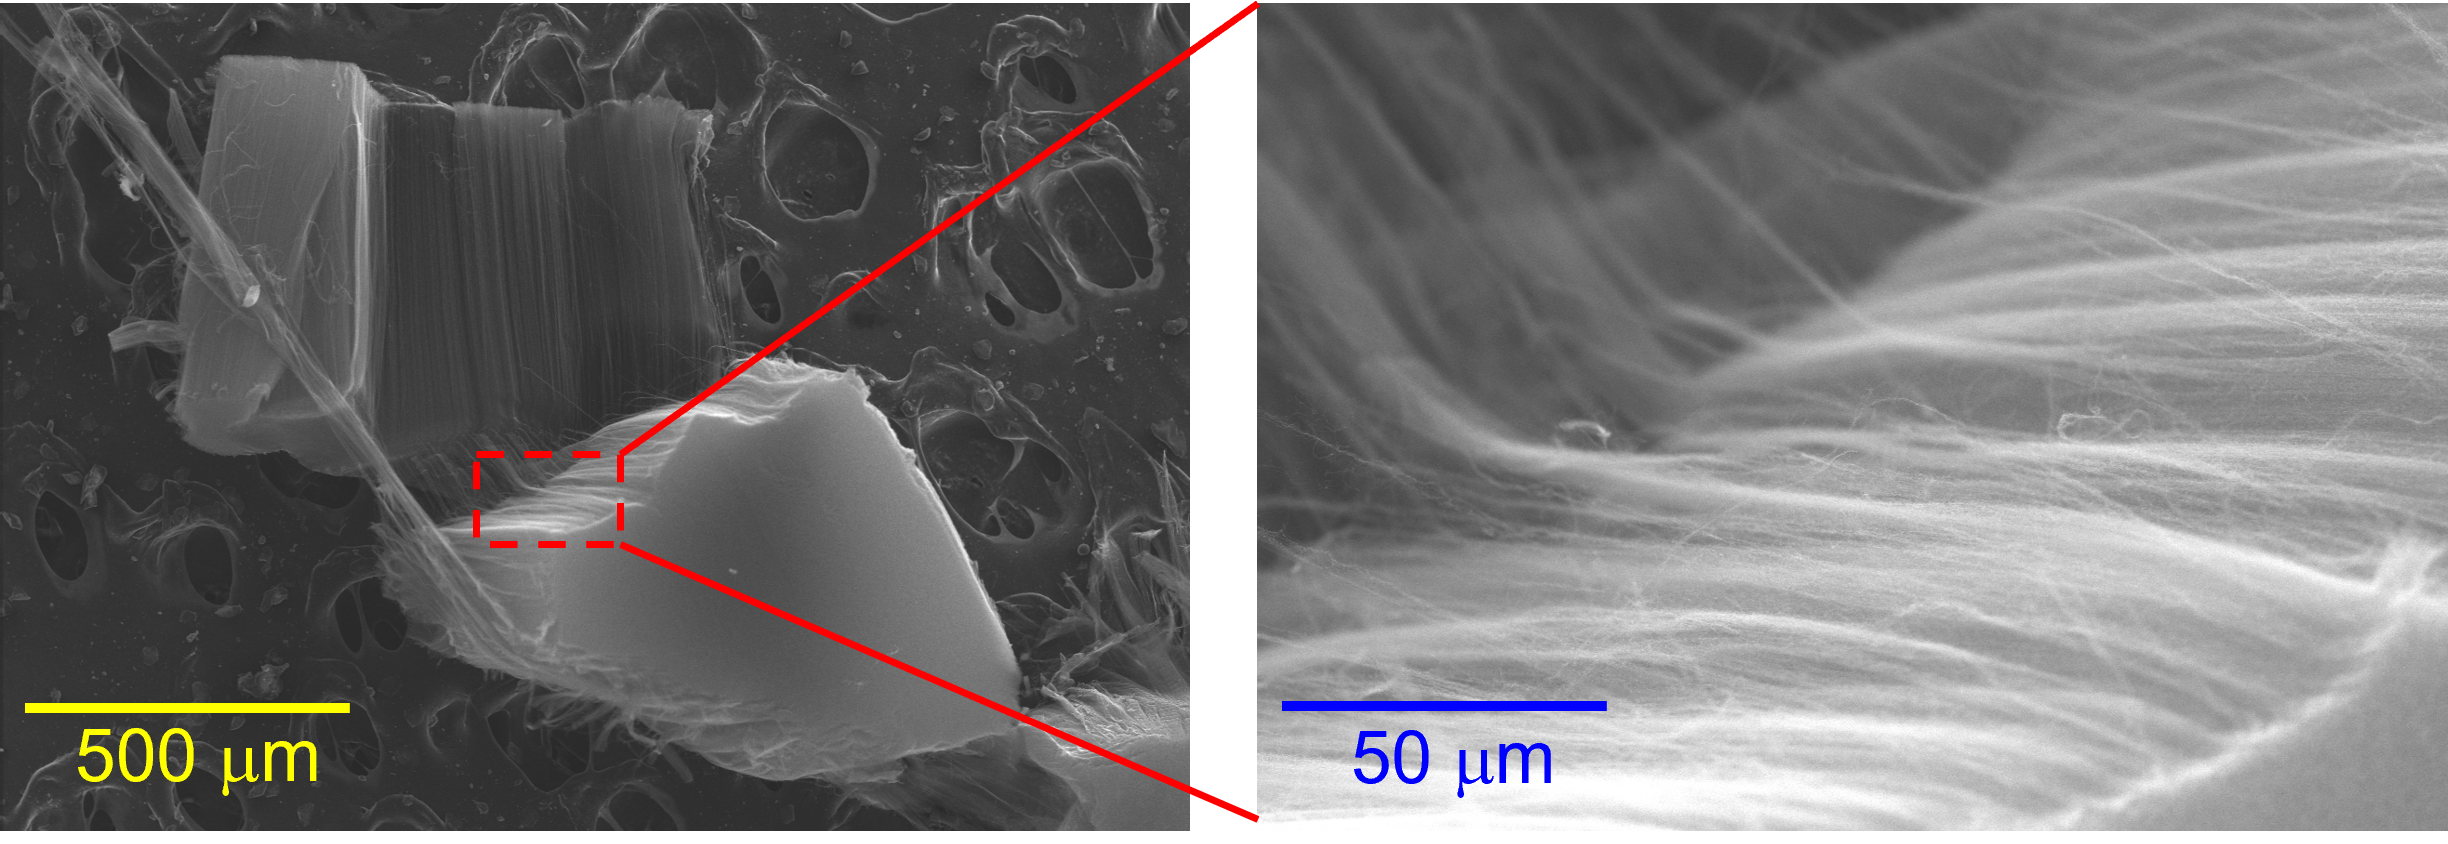
\includegraphics[keepaspectratio,width=\linewidth]{./image/1-3/1-3_CNT.png}
      \caption{
        \label{fig:1-3_CNT}
      CNTの電子顕微鏡写真。
      }
    \end{center}
  \end{figure}
  直径が数10 nmオーダの繊維状のCNTが、高指向性を持って並んで立っている様子が確認できる。
  本CNTの質量密度は0.145 g cm$^{-3}$、電子密度としてはレーザーのカットオフ密度の26倍程度と見積もられ、公表されている物性値とよく一致している。
  CNTは常温で固体であるため、実験チャンバー内に容易に導入が可能であり、かつチャンバー内でも安定して存在することが期待される。
  また、電子密度が3~26$n_{c}$($n_{c}$:レーザー波長が0.81 $\mu$mの場合の臨界密度)の領域であることから、
  プレパルスによる気化、ガス媒質としてのレーザー光の長距離伝播とそれに伴うプラズマ中での強電磁場生成とイオン加速等が相乗的に起きることが期待される。\\
  \bf{ロッド集合体}\\
  \rm
  これらの目的のもと、当研究室では、電子線リソグラフィーとプラズマエッチング技術を用いて、
  直径がサブ$\mu$mで高さが数10$\mu$mの円柱状ケイ素(シリコンロッド)が$\mu$mオーダの間隔で格子状に配置した物質(シリコンロッド集合体)を開発してきた。
  図\ref{fig:1-3_rod}は、ロッド集合体の電子顕微鏡写真である。
  \begin{figure}[H]
    \begin{center}
      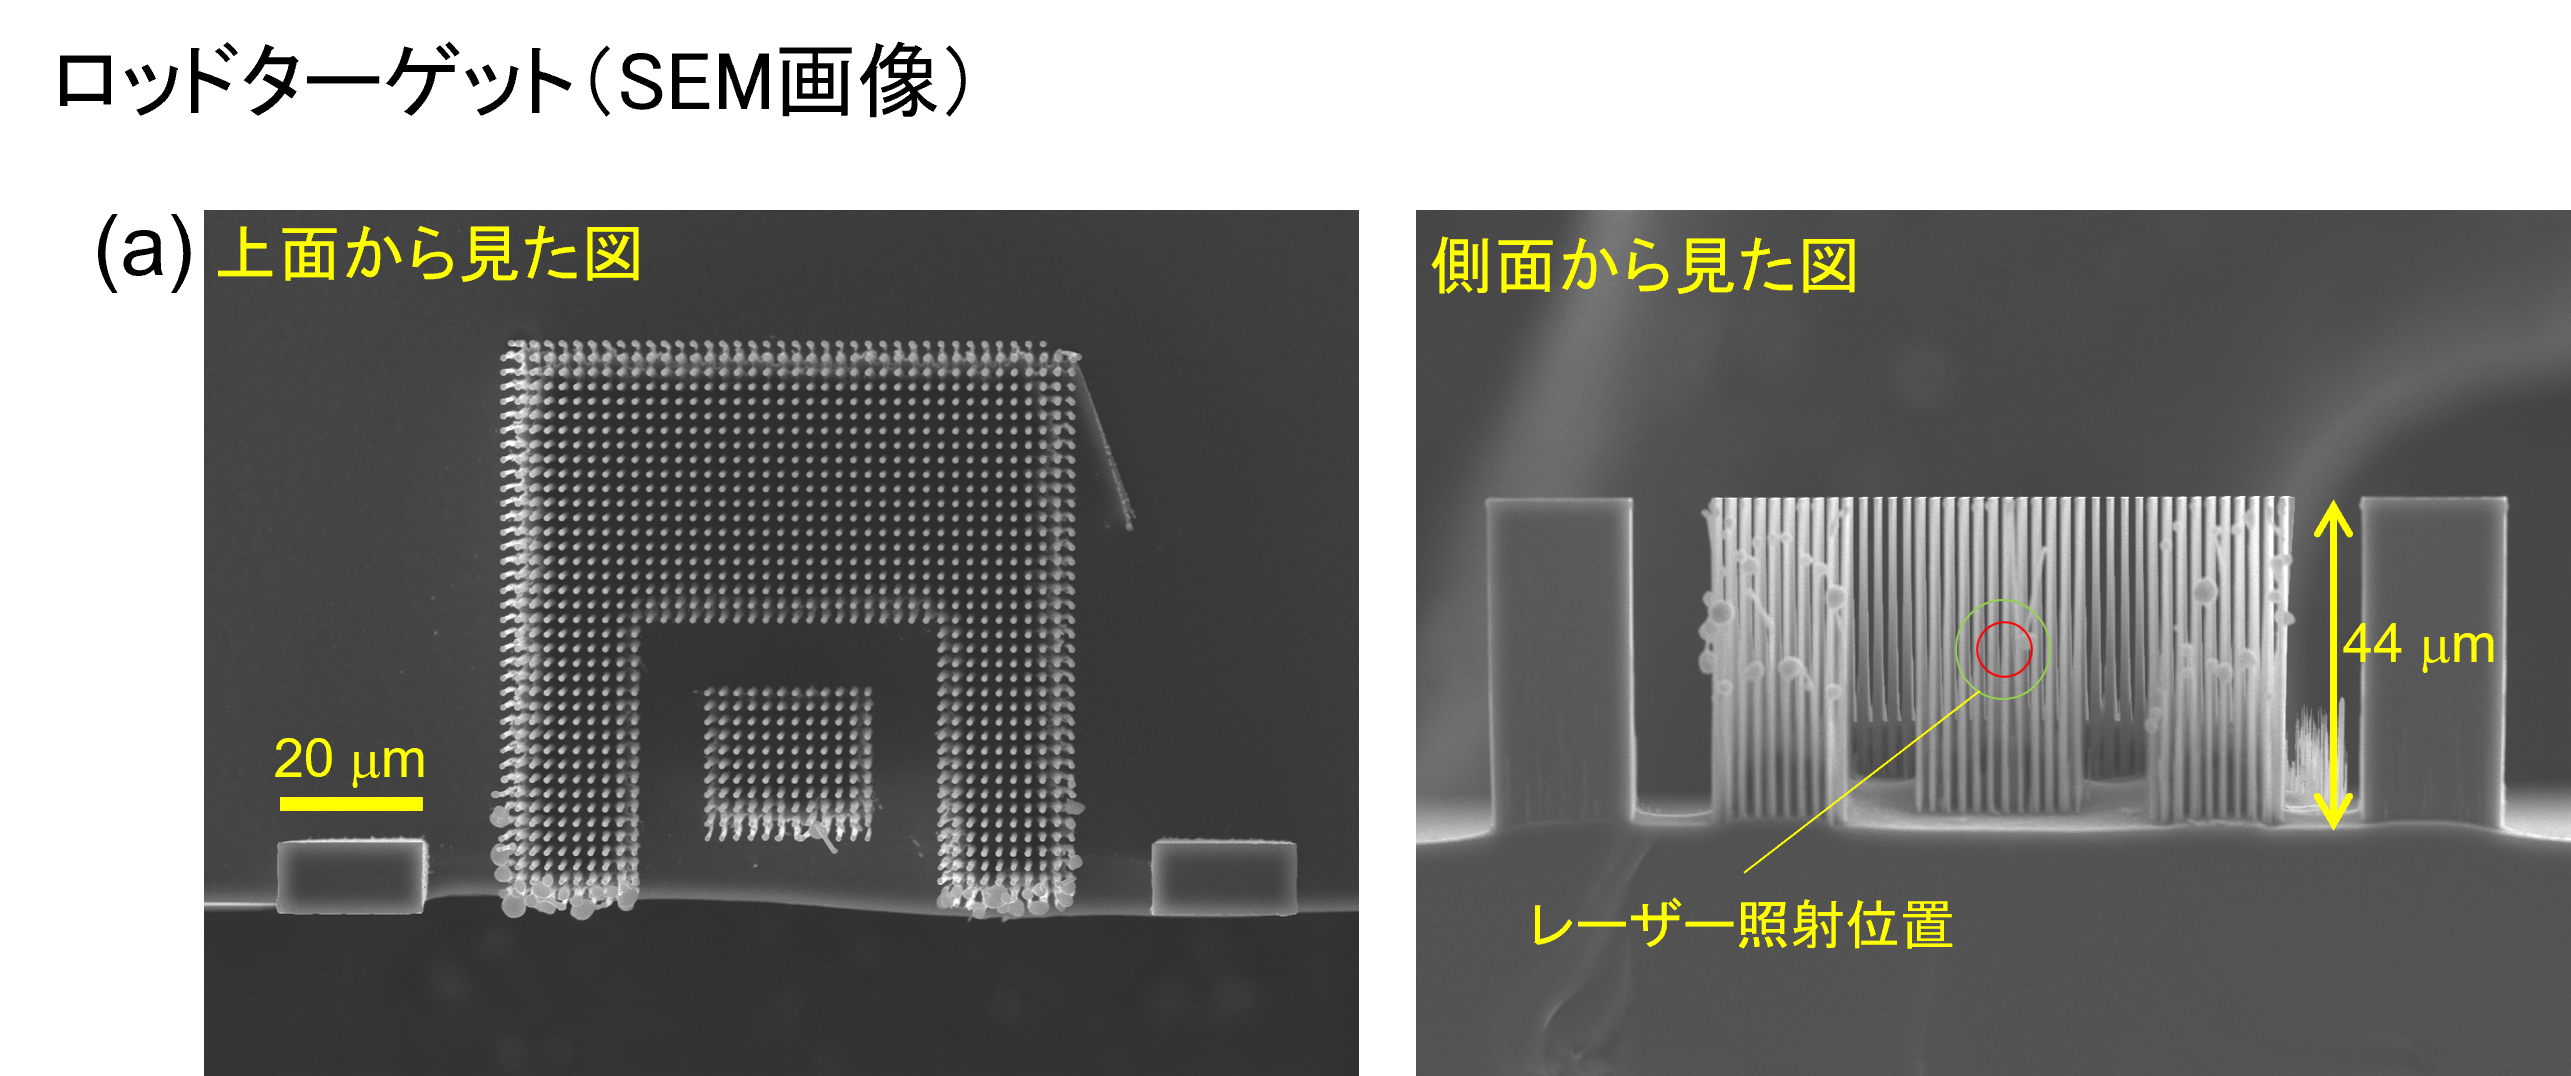
\includegraphics[keepaspectratio,width=\linewidth]{./image/1-3/1-3_rod.png}
      \caption{
        \label{fig:1-3_rod}
        rod集合体の電子顕微鏡写真。
      }
    \end{center}
  \end{figure}
  シリコンは、CNT等と比較して比熱が大きく、想定しているレーザー施設における高強度レーザーのプレパルスのエネルギーでは融解しないことが予想されている。
  我々はこれまでに、ロッド集合体を用いて、京都大学化学研究所のT6レーザー、関西光科学研究所のJ-KAREN-Pレーザー、
  理化学研究所のX線自由電子レーザーSACLAのレーザーシステムを用いて、集光強度領域が10$^{17-21}$ W/cm$^{2}$のフェムト秒極短パルス高強度レーザーを照射する実験を実施し、
  ロッド集合体の電子のエネルギー分布特性やX線小角散乱を用いたロッドの膨張速度の違い、生成する高エネルギーイオンのエネルギー特性などを調べ、
  データを蓄積してきた。図\ref{1-3_exp}は、これまでに実施してきたレーザー照射実験の概要である。
  \begin{figure}[H]
    \begin{center}
      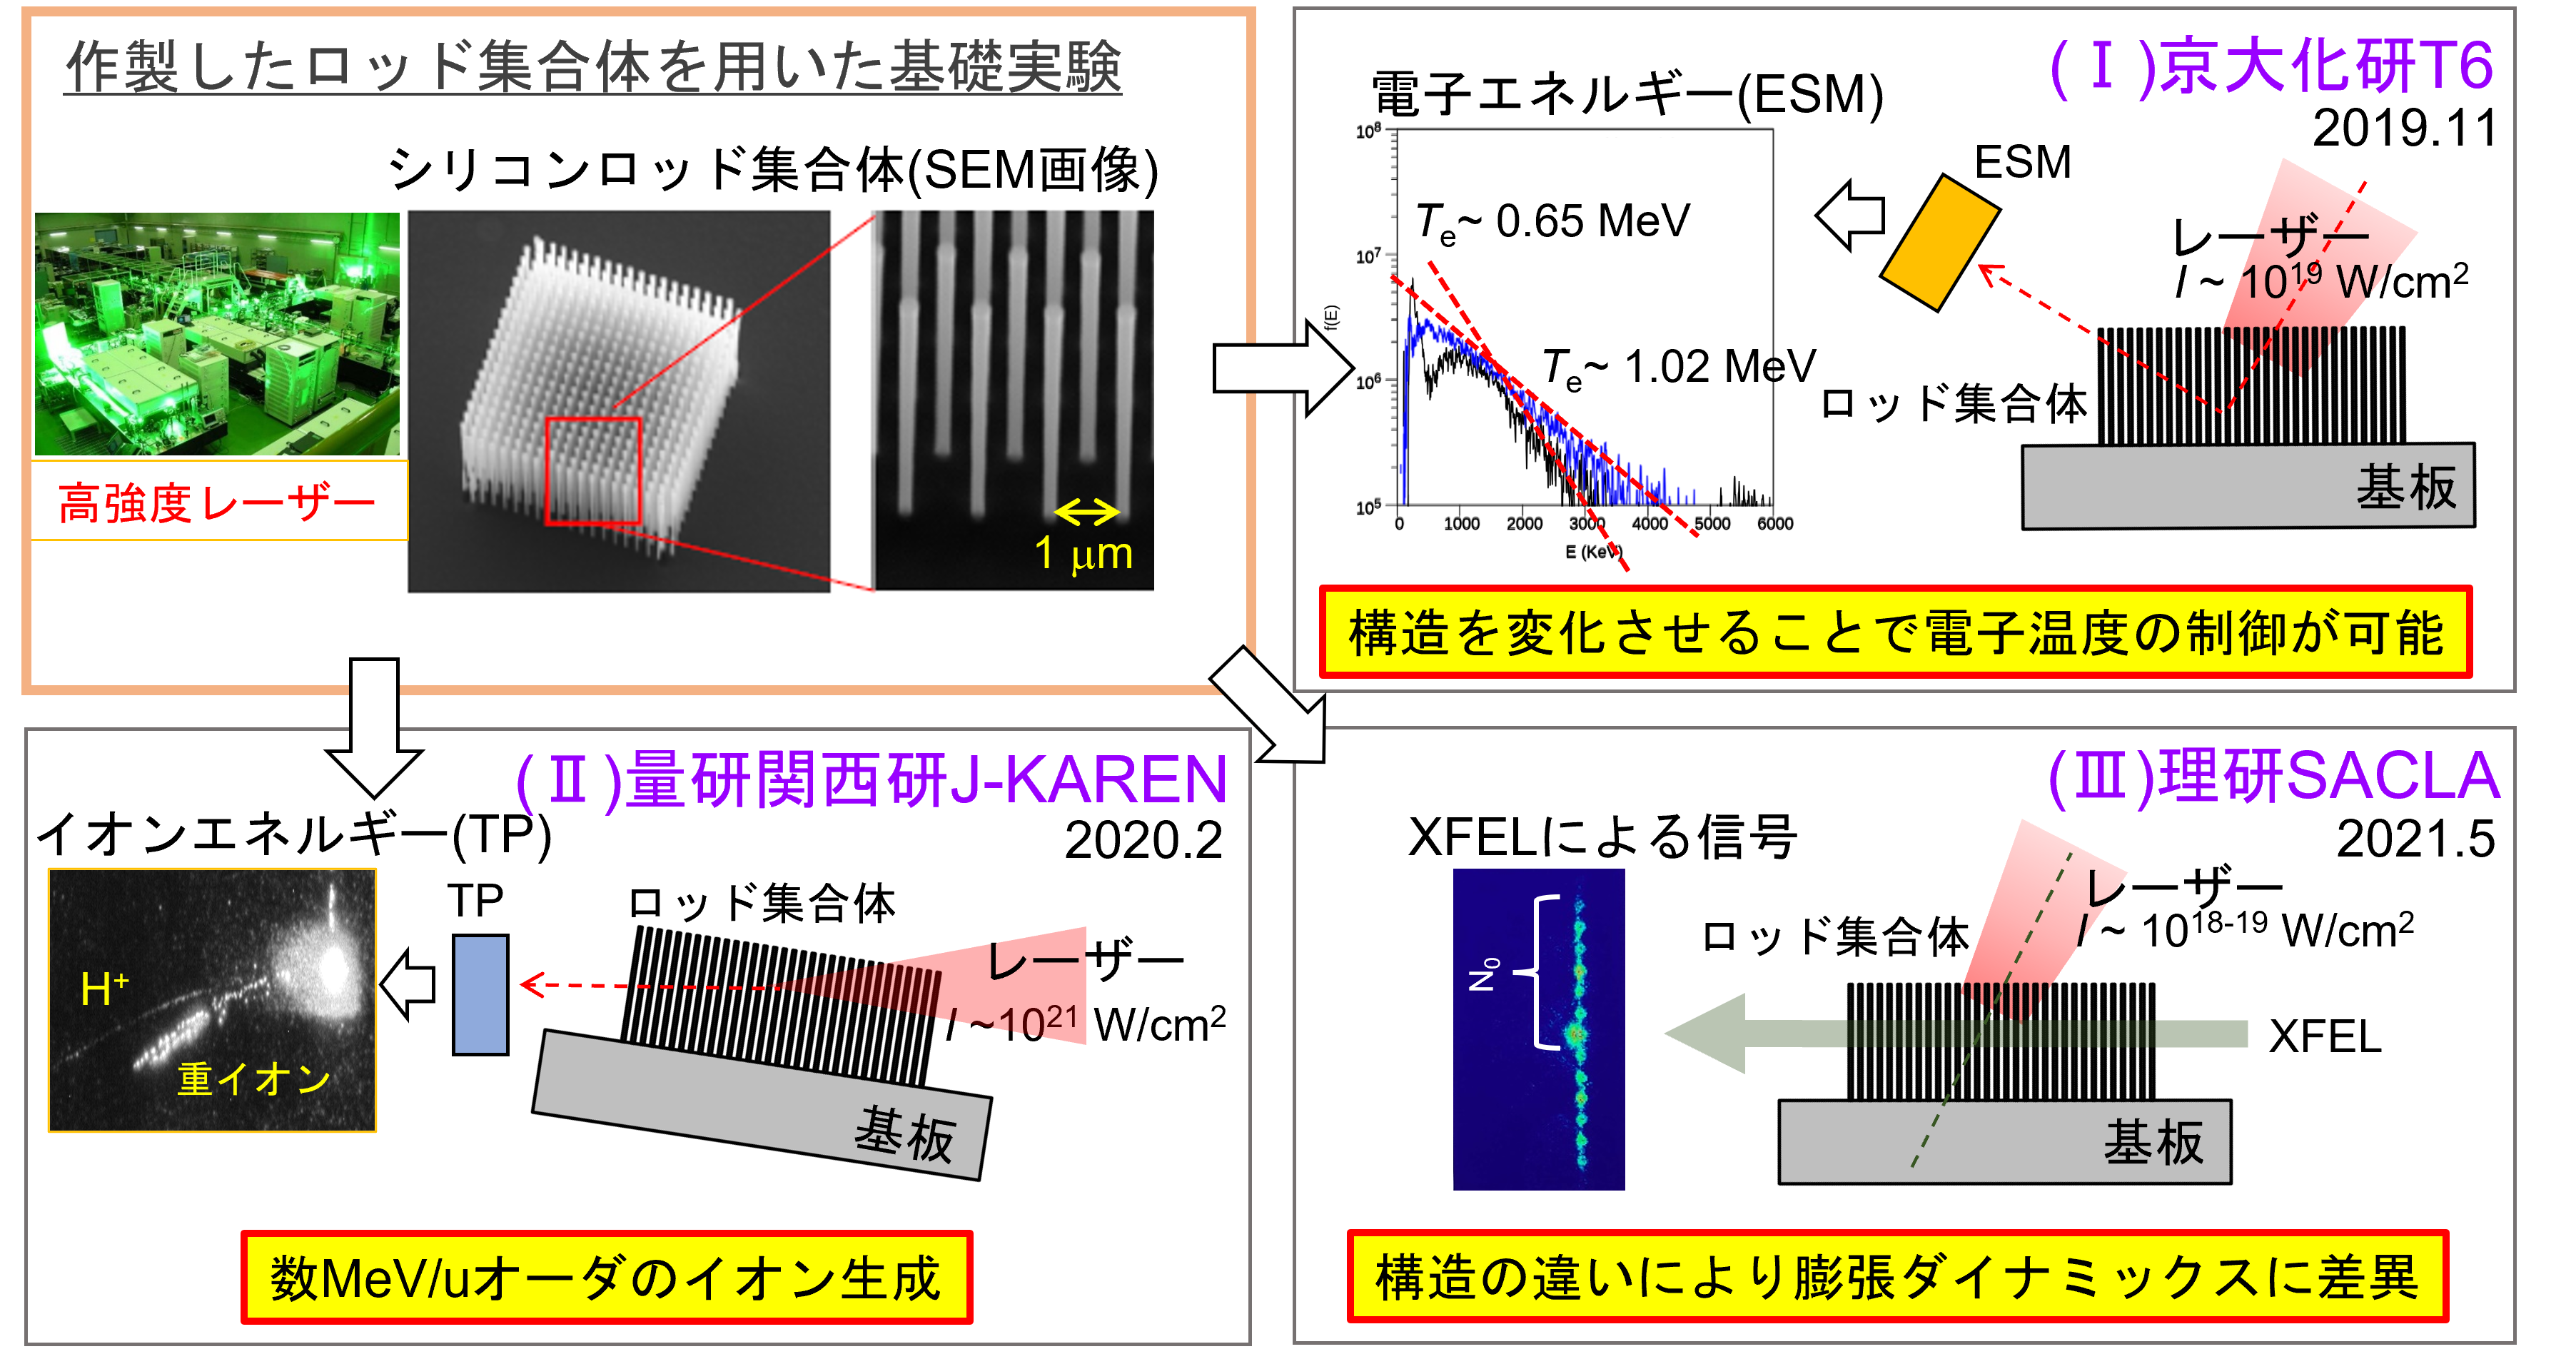
\includegraphics[scale=0.5]{./image/1-3/1-3_exp.png}      
      \caption{
        \label{1-3_exp}
      作成したロッド集合体を用いた基礎実験。
      }
    \end{center}
  \end{figure}
  その結果、(i)スラブ状のシリコン基板のみの場合と、(ii)シリコンロッド集合体の場合で比較すると、高強度領域(10$^{19-21}$ W/cm$^{2}$)において、
  ロッド集合体を用いた場合に高い電子温度が観測され、ロッド集合体のレーザーエネルギー吸収率がスラブと比較して高くなることを示唆する実験結果を得た。
  また、ロッド群の空間充填率を一定に保ってロッドの直径と間隔を変化させた場合、ロッド径を小さくすることで高い電子温度が観測され、
  レーザーエネルギーの吸収率やロッドの膨張速度に差異がみられることが確認できた。
  
  \subsection{研究目的}
  集光強度が10$^{18-20}$ W/cm$^2$領域の高強度レーザーと物質との相互作用において、サブµmオーダで比表面積の大きな微細構造を付与した物質
  (構造性媒質として参照)をターゲットとして選択することで、圧力が数M~数10 Gbar(気圧)の高エネルギー密度プラズマを生成するとともに、
  この過程で現出するTV/mオーダの強電場と kTオーダの強磁場を制御することでプラズマに自己組織化機能を発現させることが可能となる。
  これにより、高エネルギー密度プラズマの慣性時間(プラズマのスケール長を音速で割った値)を超えての閉じ込め状態が実現できれば、
  これまでフェムト秒の時間領域での現象として位置付けられてきた高エネルギー密度プラズマを、
  ピコ秒~ナノ秒の時間領域での研究対象として拡張させることが可能となり、従来は実現が困難とされてきた水素・ホウ素熱核融合反応をはじめとした、
  さまざまな応用研究への展開が期待できる。  この着想に基づき、当研究室では、
  電子線リソグラフィーとプラズマエッチングプロセスを含む半導体技術によって、
  構造性媒質として直径がサブ µm で高さが数10 µm オーダの高アスペクト比の円柱状
  ケイ素(シリコンロッド)が µm間隔で多数配列した物質(ロッド集合体)を独自開発している。
  これまでに我々は、ロッド集合体を用いて、理化学研究所のX線自由電子レーザーSACLA、
  京都大学化学研究所のT6レーザー、量子科学技術研究開発機構関西科学研究所のJ-KAREN-Pレーザーを照射する実験を実施し、
  ロッド集合体の電子のエネルギー分布特性やX線小角散乱を用いたロッドの膨張速度の違い、レーザーエネルギーの吸収率などを詳細に調べてきた。
  その結果、ロッド径・空間充填率・集合体のサイズといったロッド集合体を特徴付ける各種パラメータを適切に選択することで、
  ロッドの膨張速度やエネルギー吸収特性、電子エネルギーなどを制御可能であることを明らかにしてきた。
  これを踏まえて本研究では、構造性媒質の微細構造を適切に選択することで、
  慣性時間を超えてこれを長時間“閉じ込める”方法論を開拓することを目的とする。
  この目的のもと、相対論的電磁粒子コードEPIC3D\cite{m4}を用いて、当研究室で作製したロッド集合体と高強度レーザーとの相互作用を模擬する2次元・3次元シミュレーションを実施し、
  高強度レーザーのロッド中での伝播過程、エネルギー吸収特性を明らかにする。
  また、T6レーザーやSACLAを用いて実施された実験結果との比較を行い、
  シミュレーション結果の妥当性を検証する。



  \subsection{本論文の構成}

  2章では高強度レーザーと物質の相互作用を支配する物理現象について説明する。
  最初に相対論領域(高強度レーザー領域)での電子の特徴的な運動について記述する。次に導体極板間での電磁波伝搬についても記述する。
  3章ではシミュレーションで扱う粒子コードの概要と各パラメータの規格化などについて記述する。
  また、今回ロッドの基本性質を明らかにするために用いたエネルギー保存則を記述する。
  4章では、今回行ったシミュレーション結果を記載し、その考察をする。
  側面照射を模擬した2Dシミュレーションでは、ロッド径が慣性時間伸長に寄与しうるパラメータであるかの検証、
  上面照射を模擬した2Dシミュレーションでは、基盤ターゲット及び構造を付与したターゲットにおける物理過程の差異、および伝搬過程について考察する。
  最後に3Dシミュレーションでは、エネルギー保存則を任意の分割領域に適応することで、構造性媒質の吸収特性について明らかにする。

% % input1ed
% \begin{thebibliography}{99}
% \bibitem{Kiriyama2015}
% H. Kiriyama $et\ al.,$ IEEE J. Sel. Top. Quantum Phys. {\bf 21}(1), 232-249 (2015). 
% \bibitem{AlexOE2017}
% A. S. Pirozhkov $et\ al.,$ Opt. Express {\bf 25}(17), 20486 (2017). 
% \bibitem{Kiriyama2018}
% H. Kiriyama $et\ al.,$ Optics Letters {\bf 43}, 2595 (2018).
% \bibitem{Kiriyama2020}
% H. Kiriyama $et\ al.,$ Optics Letters {\bf 45}, 1100 (2020).
% \end{thebibliography}
% \newpage

\end{document}

